\documentclass[12pt]{article}

\usepackage{fullpage}
\usepackage{pdfpages}
\usepackage[round]{natbib}
\usepackage{multirow}
\usepackage{booktabs}
\usepackage{graphicx}
\usepackage{float}

\newcounter{acnum}
\newcommand{\actheacnum}{AC\theacnum}
\newcommand{\acref}[1]{AC\ref{#1}}

\newcounter{ucnum}
\newcommand{\uctheucnum}{UC\theucnum}
\newcommand{\uref}[1]{UC\ref{#1}}

\newcounter{mnum}
\newcommand{\mthemnum}{M\themnum}
\newcommand{\mref}[1]{M\ref{#1}}

\begin{document}

\title{Design Document for Snake Game} 
\author{Keyur Patel
Alex Guerrero
Shafeeq Rabbani}
\date{\today}
	
\maketitle

\tableofcontents

\newpage

\section{Introduction}

The following documentation is intended elaborate how the design of the snake game is implemented. The document will also explain how the functional and non-functional requirements mentioned in the Software Requirements Specification will be explained. This document is intended for the following readers:

\begin{itemize}
\item Designers: The document can serve to ensure that all functional and non-functional requirements are met. Further, designers can also use this document to verify any discrepancies among different modules.

\item New Project Members: This document can bring new team members up-to-date with the overview and structure of the game.

\item Maintainers: This document can also used to understand the structure of the game and all of the modules within. It would then be the responsibility of the maintainers to update the Design document by mentioning any change they have made to it.

\item Professor and TAs: As this document is being marked, the professors and TAs will have access to the document to determine if it was structured as intended. The document will also serve to give the Professor and the TAs an overview of the modules of the snake game.
\end{itemize}

The Snake game has been divided up into modules which hide information from other modules in the document in order to implement the Information Hiding principle of Software Engineering. Further, the modules only share the information amongst each other that is necessary. This is done to ensure the Low Coupling principle of Software Engineering. In order to read or modify values within different modules, there are getter and setter methods unique to the respective modules. This is done to implement the Encapsulation principle of Software Engineering.

This document consists of the Module Interface Specification (or MIS) which is intended for programmers who work to further develop the Snake Game.

The rest of this document consists of the GANTT and PERT chart meant to highlight the time frame for future deliverables for development of the Snake Game.

\section{Anticipated and Unlikely Changes} \label{SecChange}

There are two types of possible changes: Anticipated and Unlikely Changes. This section covers both of these changes.

\subsection{Anticipated Changes} \label{SecAchange}



\begin{description}
\item[\refstepcounter{acnum} \actheacnum \label{acFood}:] The type of food which the snake eats.
\item[\refstepcounter{acnum} \actheacnum \label{acGameOver}:] What must happen after the game is over.
\item[\refstepcounter{acnum} \actheacnum \label{acMainMenu}:] More options available in the menu as game expands .e.g. save game, high scores, sound, difficulty etc.
\item[\refstepcounter{acnum} \actheacnum \label{acPlayMap}:] The map of the game.
\item[\refstepcounter{acnum} \actheacnum \label{acPowerUps}:] Different PowerUps will be available such as Intangibility (.i.e. ability to go through walls) as the game expands.
\item[\refstepcounter{acnum} \actheacnum \label{acSnake}:] The characteristics of the snake .e.g. its color, the way it grows, the speed at which it moves etc.
\item[\refstepcounter{acnum} \actheacnum \label{acInput}:] Addition or modification of Keyboard and mouse commands as game is expanded in the future.
\end{description}

\subsection{Unlikely Changes} \label{SecUchange}

These are design decisions that have to be changed after they were fixed in the software architecture state (in order to simplify the design). It wasn't intended that these decisions would have to be changed.

\begin{description}
\item[\refstepcounter{ucnum} \uctheucnum \label{ucIO}:] Input/Output devices
  (Input: Keyboard, Mouse Output: Screen).
\item[\refstepcounter{ucnum} \uctheucnum \label{ucPygame}:] The game will always be implemented in python using the Pygame library.
\item[\refstepcounter{ucnum} \uctheucnum \label{ucGoal}:] The goal of the game is to get the highest score possible.
\end{description}

\section{Module Hierarchy} \label{SecMH}

This section lists the modules in the Snake game. The modules listed below are leaves in the module hierarchy in the table below. 

\begin{description}
\item [\refstepcounter{mnum} \mthemnum \label{mFood}:] Food Module
\item [\refstepcounter{mnum} \mthemnum \label{mGameOver}:] GameOver Module
\item [\refstepcounter{mnum} \mthemnum \label{mMainMenu}:] MainMenu Module
\item [\refstepcounter{mnum} \mthemnum \label{mPlayMap}:] PlayMap Module
\item [\refstepcounter{mnum} \mthemnum \label{mPowerUp}:] PowerUp Module
\item [\refstepcounter{mnum} \mthemnum \label{mSnake}:] Snake Module
\item [\refstepcounter{mnum} \mthemnum \label{mController}:] Controller Module
\end{description}

The Hardware-Hiding Module is already implemented by the operating system and hence will not be reimplemented.

\begin{table}[h!]
\centering
\begin{tabular}{p{0.3\textwidth} p{0.6\textwidth}}
\toprule
\textbf{Level 1} & \textbf{Level 2}\\
\midrule

{Hardware-Hiding Module} & ~ \\
\midrule

\multirow{7}{0.3\textwidth}{Behaviour-Hiding Module} 
& Food Module\\
& GameOver Module\\
& MainMenu Module\\
& PlayMap Module\\
& PowerUp Module\\ 
& Snake Module\\
& Controller Module\\
\midrule

{Software Decision Module} & ~ \\
\bottomrule

\end{tabular}
\caption{Module Hierarchy}
\label{TblMH}
\end{table}

\section{Connection Between Requirements and Design} \label{SecConnection}

The table below highlights the connection between the system requirements(which are listed in the Software Requirements Specification) and the modules.

\begin{table}[H]
\centering
\begin{tabular}{p{0.2\textwidth} p{0.6\textwidth}}
\toprule
\textbf{AC} & \textbf{Modules}\\
\midrule
AC1 & M1\\
AC2 & M2\\
AC3 & M3\\
AC4 & M4\\
AC5 & M5\\
AC6 & M6\\
AC7 & M7\\
\bottomrule
\end{tabular}
\caption{Trace Between Anticipated Changes and Modules}
\end{table}

\section{Module Decomposition} \label{SecMD}


\subsection{Behaviour-Hiding Module}

\begin{description}
\item[Secrets:]The contents of the required behaviours.
\item[Services:]Includes programs that provide externally visible behaviour of
  the system as specified in the software requirements specification (SRS)
  documents. This module serves as a communication layer between the
  hardware-hiding module and the software decision module. The programs in this
  module will need to change if there are changes in the SRS.
\end{description}

\subsubsection{Food (M1)}


\begin{description}

\item[Secrets:] The generation of food location.
\item[Services:] Places food in a random location on the play map.
\item[Implemented By:] SWHS
\item[Secrets:]The structure of the Food
\item[Services:]generates and stores a Food object in a random position

\end{description}

\subsubsection{GameOver Module (M2)}


\begin{description}

\item[Secrets:]The format and structure of the Power up
\item[Services:]generates and stores a powerup object in a random position
\item[Implemented By:] SWHS
\end{description}

\subsubsection{MainMenu Module (M3)}

\begin{description}



\item[Secrets:] The format of the game board
\item[Services:] updates state of the game board and returns objects to be displayed
\item[Implemented By:] SWHS
\end{description} 

\subsubsection{PlayMap Module (M4)}


\begin{description}
\item[Secrets:] The format and and state update redirection of the backend
\item[Services:] emulates the game window and different states and menus
\item[Implemented By:] SWHS
\end{description} 

\subsubsection{PowerUp Module (M5)}


\begin{description}

\item[Secrets:] The behaviour of the Snake object
\item[Services:] defines the points of the snake and has functions to manipulate snake
\item[Implemented By:] SWHS

\end{description} 
 
\subsubsection{Snake Module (M6)}

\begin{description}
\item[Secrets:] Attributes pertaining to the snake such as its length.
\item[Services:] Determines the speed the snake moves at, its length etc.
\item[Implemented By:] SWHS
\end{description}

\subsubsection{Controller Module (M7)}

\begin{description}
\item[Secrets:] The algorithm for coordinating the running of the program.
\item[Services:] Provides the main program.
\item[Implemented By:] SWHS
\end{description}

\section{Traceability Matrix} \label{SecTM}

This section shows the traceability matrix between the modules and the
requirements.

% the table should use mref, the requirements should be named, use something
% like fref
\begin{table}[H]
\centering
\begin{tabular}{p{0.2\textwidth} p{0.6\textwidth}}
\toprule
\textbf{Req.} & \textbf{Modules}\\
\midrule
R1 & M2\\
R2 & M2, M8\\
R3 & M2,M5,M6,M7\\
R4 & M3, M6, M7\\
R5 & M2\\
R6 & M2,M5,M6,M7\\
R7 & M2,M3,M4,M5,M6\\
R8 & M2,M4, M5\\
\bottomrule
\end{tabular}
\caption{Trace Between Requirements and Modules}
\label{TblRT}
\end{table}

\section{Use Hierarchy Between Modules} \label{SecUse}

In this section, the uses hierarchy between modules is
provided.
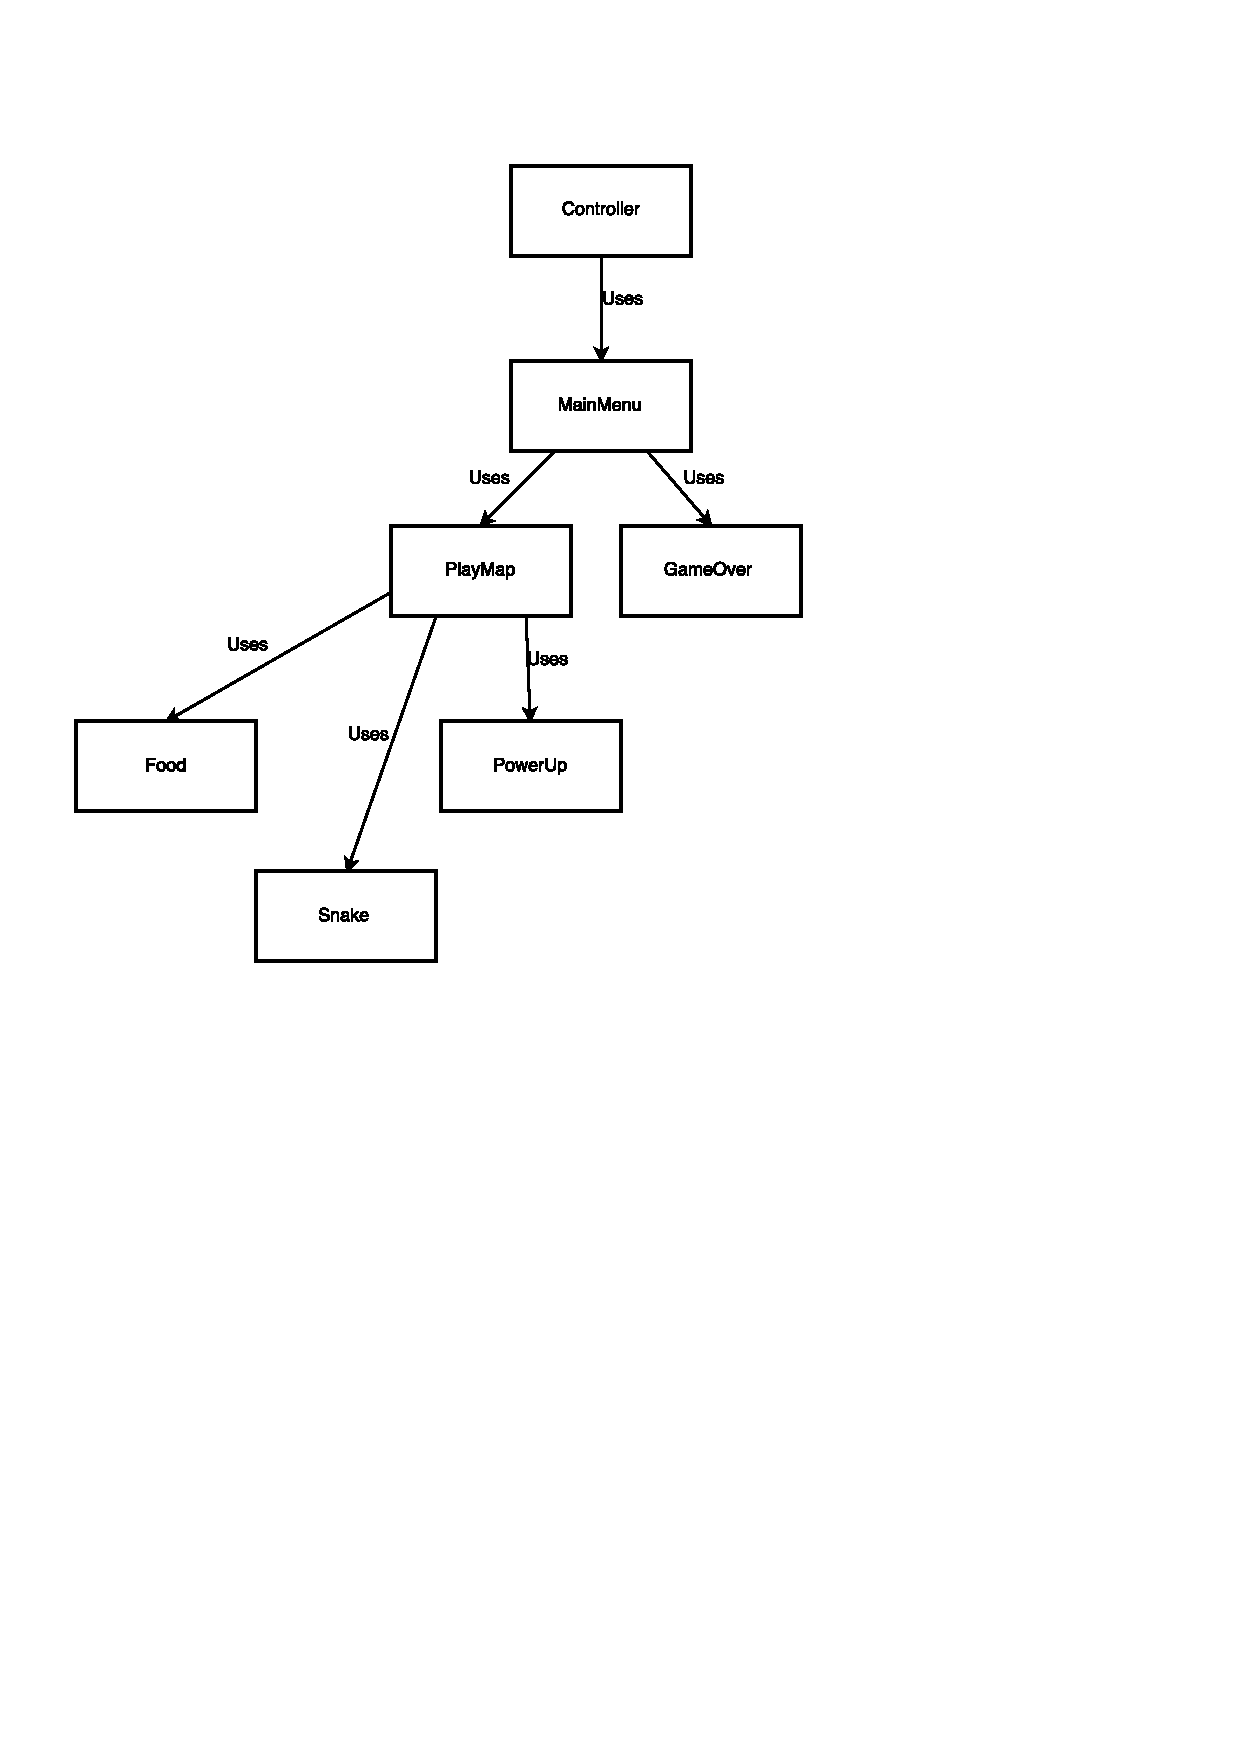
\includepdf[pages={1}]{UsesHeirarchy.pdf}


\section{Course Schedule} 

In this section, a Gantt and PERT Chart scheduling the remainder of the semester are provided.
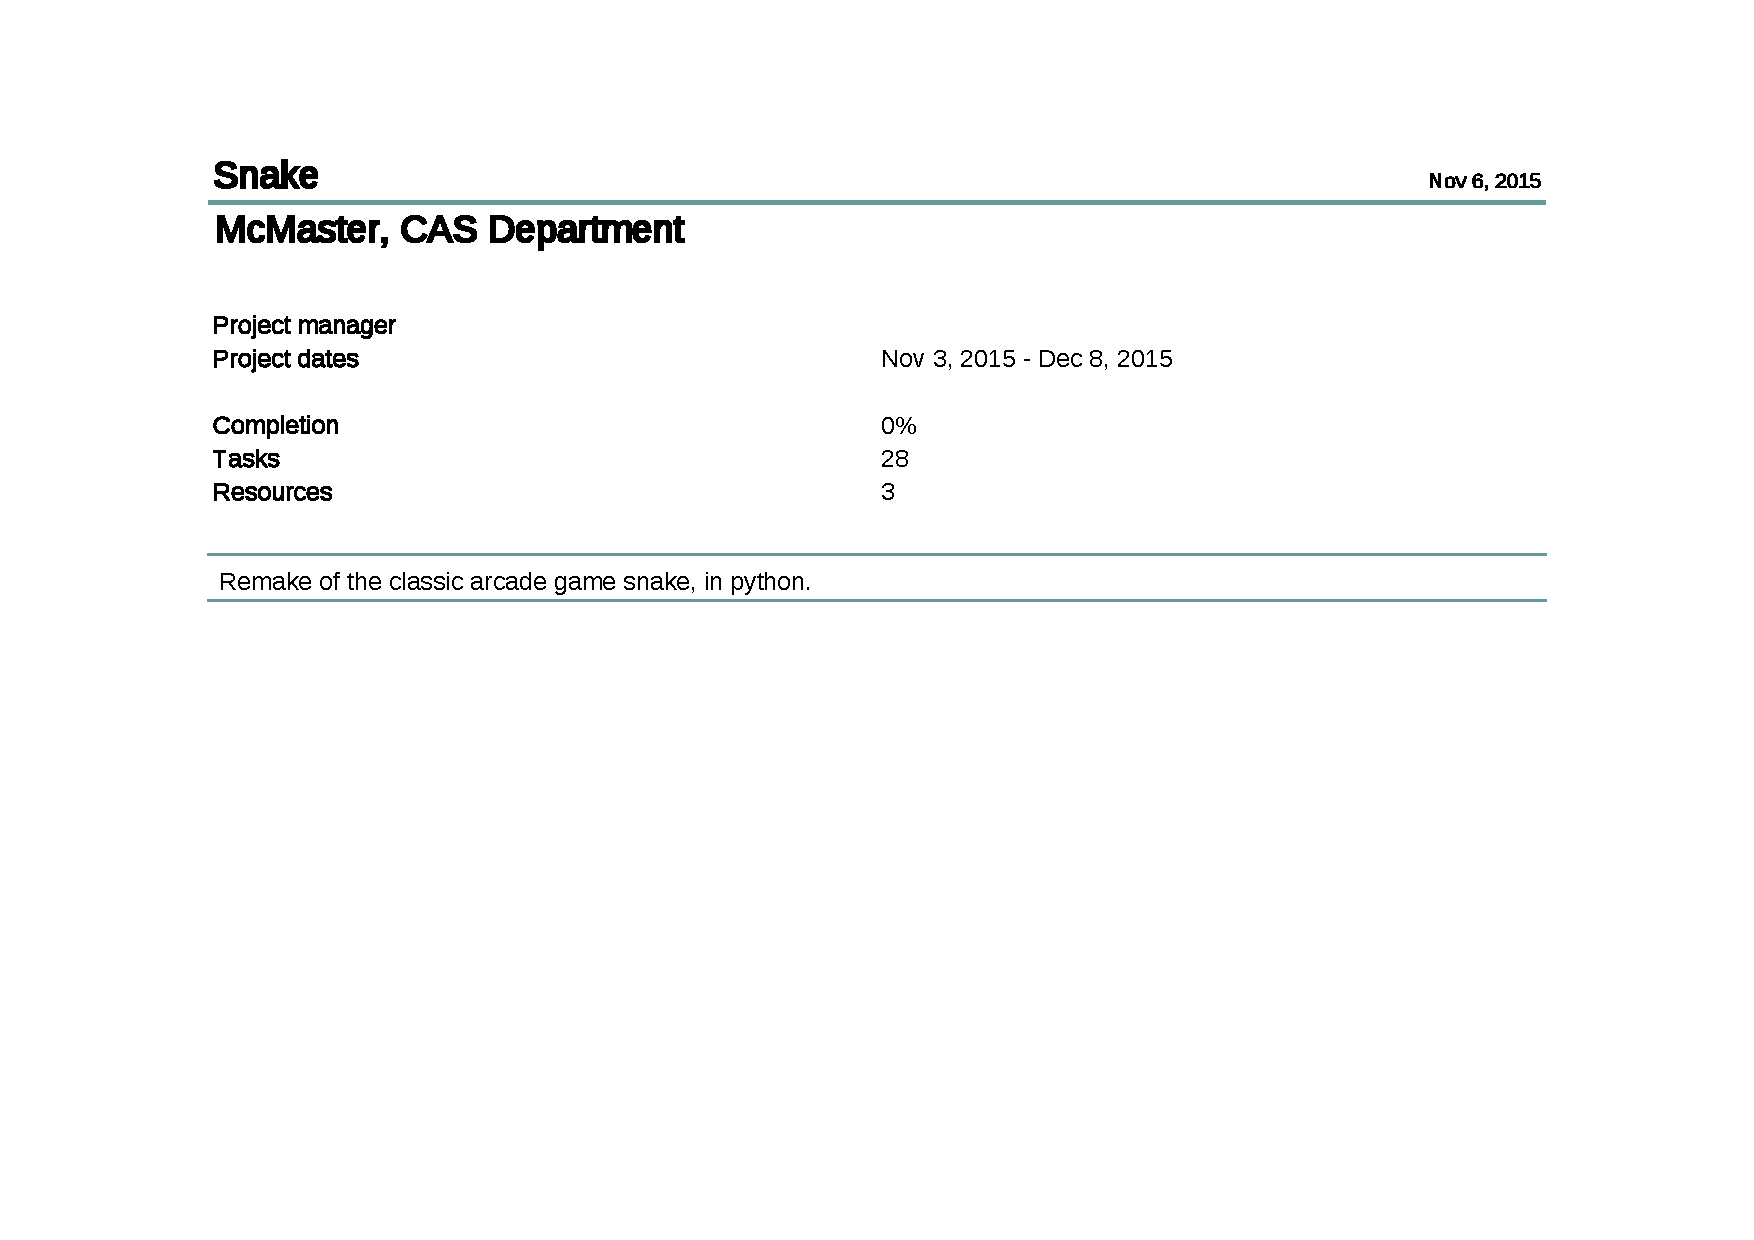
\includepdf[pages={1,2,3,4,5,6}]{GanttChart.pdf}
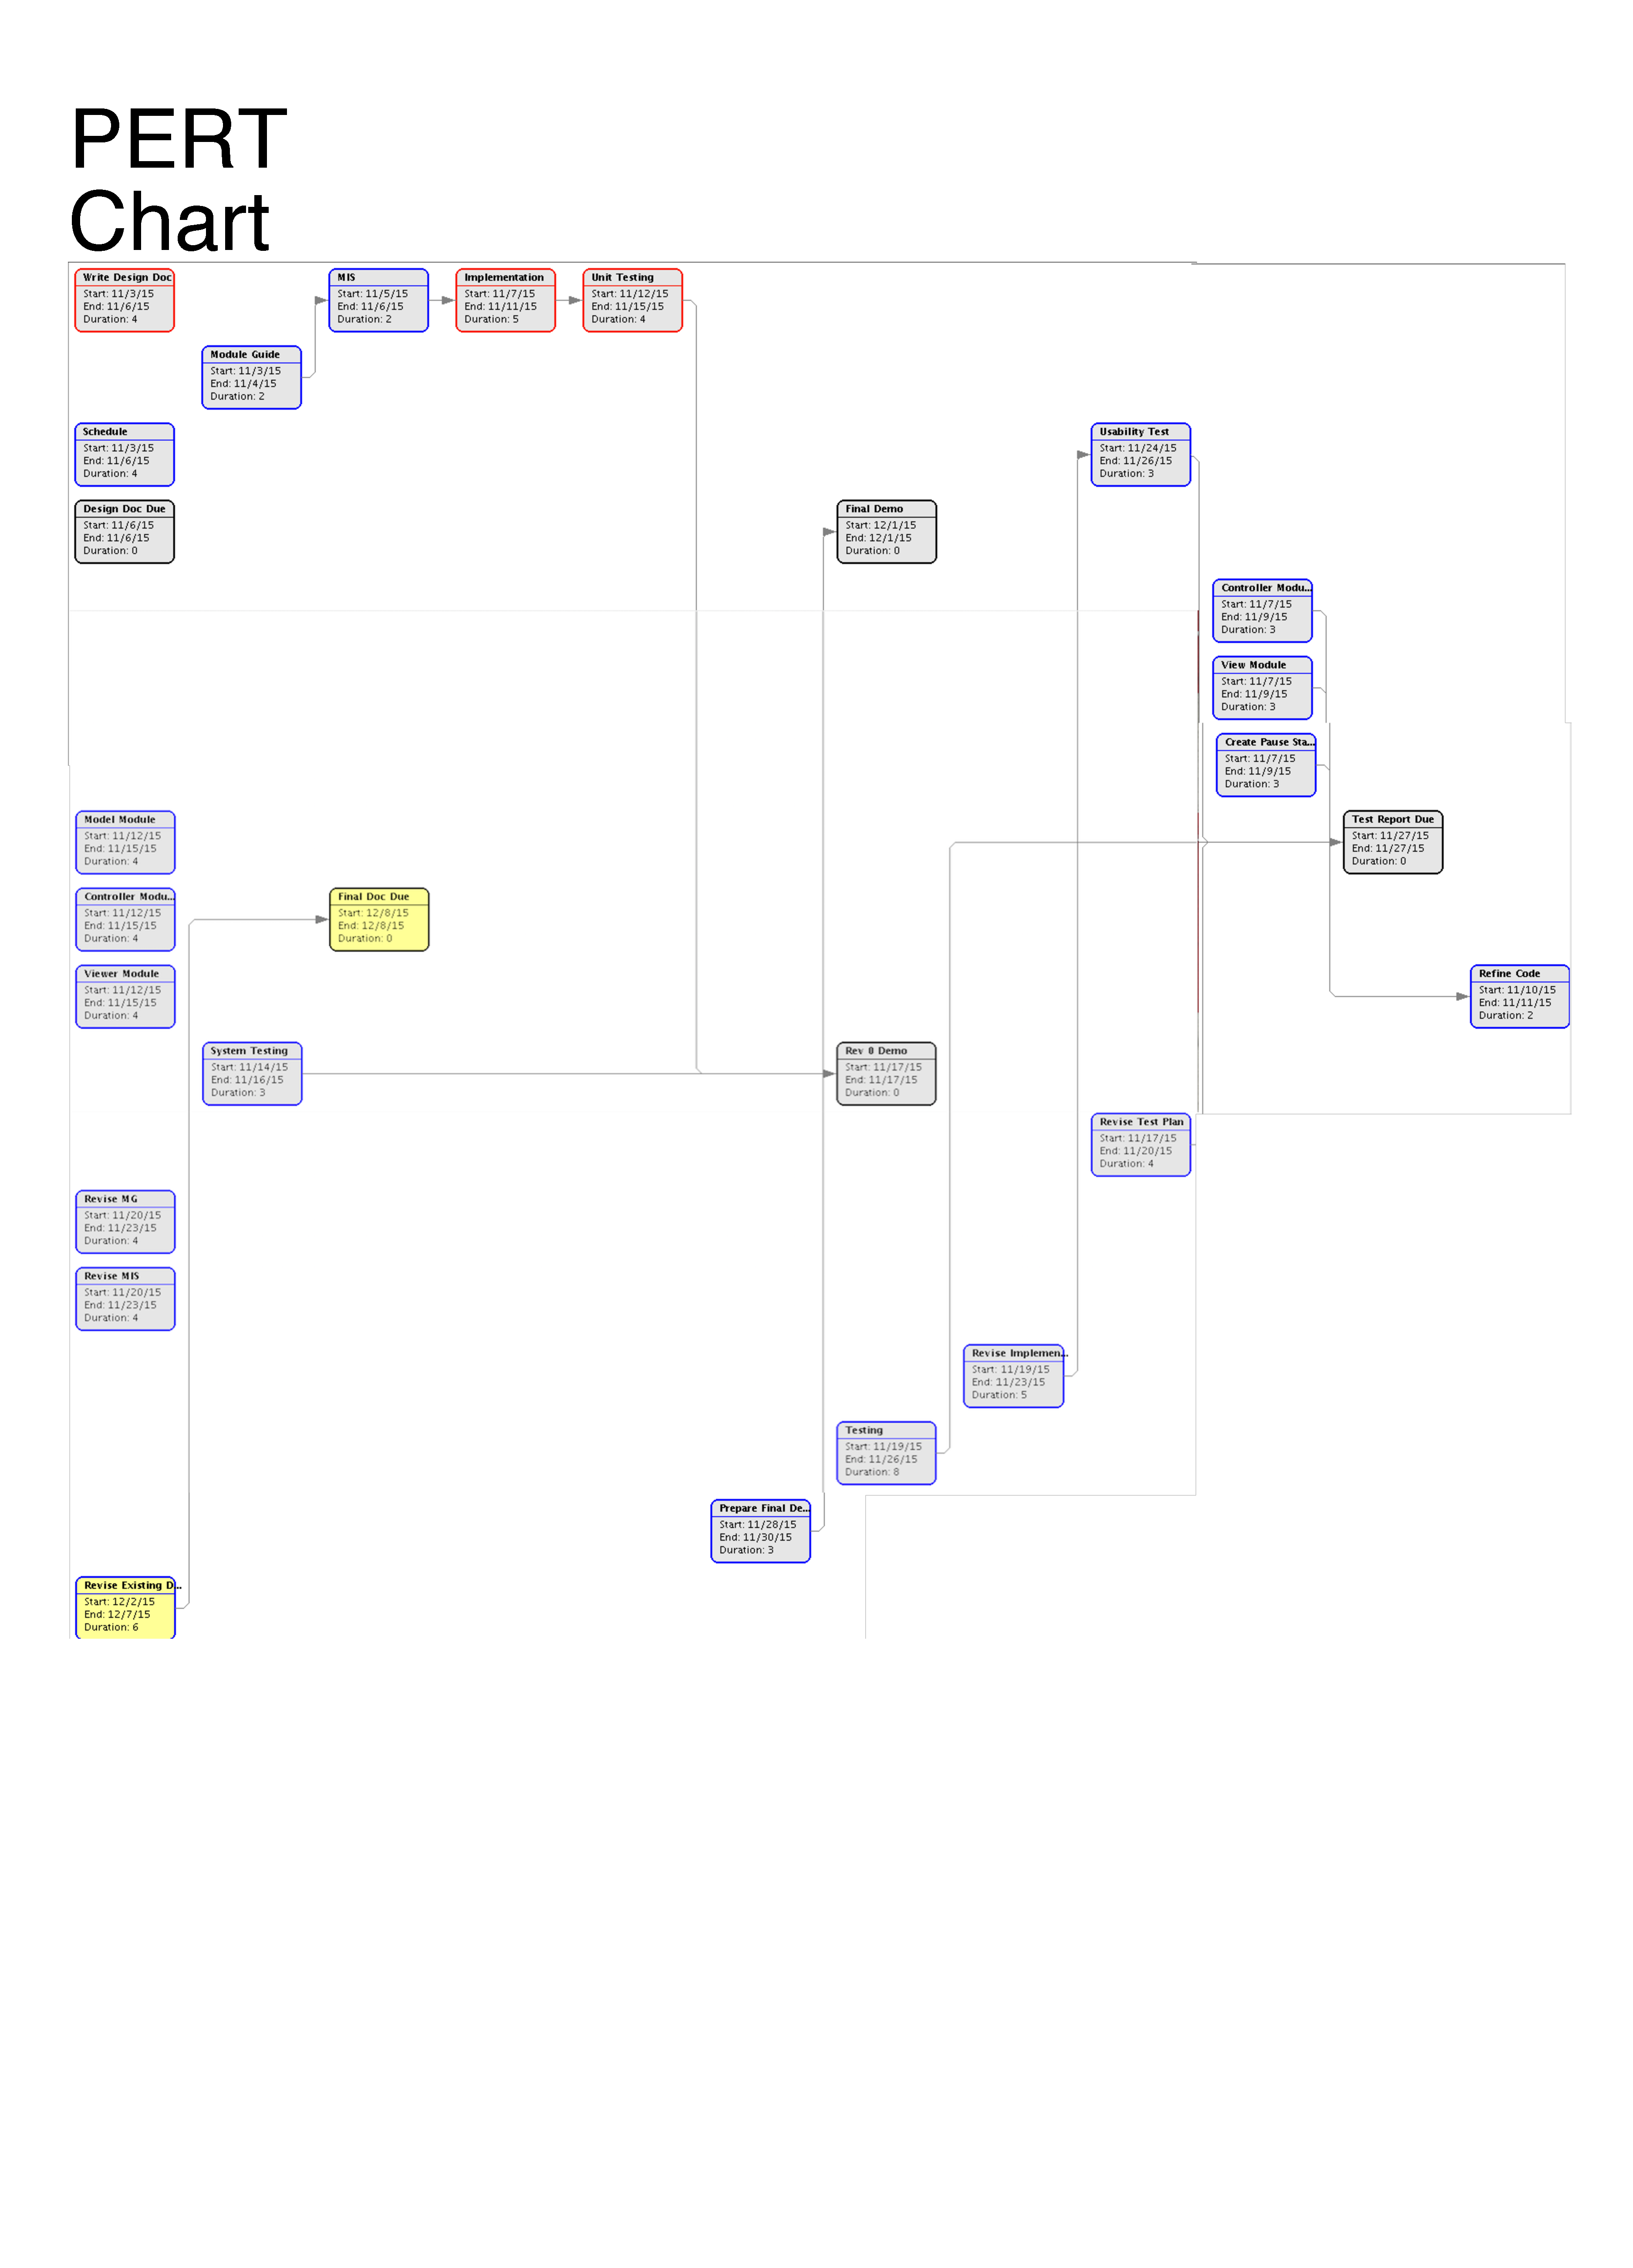
\includepdf[pages={1}]{PERTChart.pdf}


%\section*{References}

\bibliographystyle {plainnat}
\bibliography {../PCM_SRS/PCM_SRS}

\end{document}
